\documentclass[12pt]{article}
\usepackage[margin=2.5cm]{geometry}
\usepackage{enumerate}
\usepackage{amsfonts}
\usepackage{amsmath}
\usepackage{fancyhdr}
\usepackage{amsmath}
\usepackage{amssymb}
\usepackage{amsthm}
\usepackage{mdframed}
\usepackage{graphicx}
\usepackage{subcaption}
\usepackage{listings}
\usepackage{xcolor}
\usepackage[utf]{kotex}

\definecolor{codegreen}{rgb}{0,0.6,0}
\definecolor{codegray}{rgb}{0.5,0.5,0.5}
\definecolor{codepurple}{rgb}{0.58,0,0.82}
\definecolor{backcolour}{rgb}{0.95,0.95,0.92}

\lstdefinestyle{mystyle}{
    backgroundcolor=\color{backcolour},
    commentstyle=\color{codegreen},
    keywordstyle=\color{magenta},
    numberstyle=\tiny\color{codegray},
    stringstyle=\color{codepurple},
    basicstyle=\ttfamily\footnotesize,
    breakatwhitespace=false,
    breaklines=true,
    captionpos=b,
    keepspaces=true,
    numbers=left,
    numbersep=5pt,
    showspaces=false,
    showstringspaces=false,
    showtabs=false,
    tabsize=1
}

\lstset{style=mystyle}

\begin{document}
\title{CSC148 Worksheet 7 Solution}
\author{Hyungmo Gu}
\maketitle

\section*{Question 1}

\begin{itemize}
    \item Noticed that there are 11 students in total.
    \item Students should be grouped by year as closest as possible.
\end{itemize}

\bigskip

\textbf{Notes:}

\begin{itemize}
    \item 형모 해낼 뚜 있쬬!
    \item 형모 화이팅!
\end{itemize}

\section*{Question 2}
\begin{center}
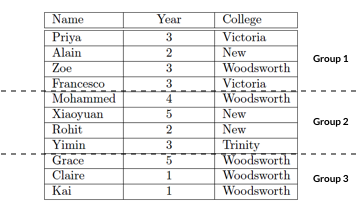
\includegraphics[width=0.7\linewidth]{images/worksheet_7_q2_solution.png}
\end{center}

\section*{Question 3}
\begin{itemize}
    \item

    First, we need to find the group as homogenous as possible in terms of year students
    are in.

    \bigskip

    The definition tells us group needs to be in 4,
    and the following table tell us there are 4 $3^{rd}$ year students.

    \bigskip

    \begin{center}
        \begin{tabular}{|c|c|}
            \hline
            Student Year & Number of Students\\
            \hline
            1 & 2\\
            \hline
            2 & 2\\
            \hline
            3 & 4\\
            \hline
            4 & 1\\
            \hline
            5 & 2\\
            \hline
        \end{tabular}
    \end{center}

    \bigskip

    It follows from these facts that the group of $3^{rd}$ year students best satisfy
    this criterion.

    \bigskip

    Next, we need to find the group as not homogenous as possible in terms of year students
    are in.

    \bigskip

    The same table tells us with 2 $5^{th}$ year students, 1 $4^{th}$
    year students and 1 $3^{rd}$ year student, a group spanning 3 years can be
    created.

    \bigskip

    Since we know there can't be a group spanning 4 years, we can conclude the
    group of 3 years (2 $5^{th}$ year students, 1 $4^{th}$ year students and 1
    $3^{rd}$ year student) best satisfy this criterion.

\end{itemize}

\section*{Question 4}
\begin{itemize}
    \item

    We will calculate the group score based on the code below. The code
    is also included in \textit{worksheet\_7\_q4\_solution.py}

    \bigskip

    \begin{lstlisting}[language=Python]
    def get_group_score(group):
        """Evaluates the group score

            Precondition: len(group) == 4
        """
        n = 4

        max_year = get_max_year(group)
        min_year = get_min_year(group)
        similarity_list = []

        i = 0

        while i < 4:
            j = 0
            while j < 4:
                # find the scaled distance
                scaled_distance = 0
                if max_year != min_year:
                    scaled_distance = abs(group[i]['year'] - group[j]['year']) / float(max_year - min_year)

                # find the similarity
                similarity = 1 - scaled_distance

                # add to list
                similarity_list.append(similarity)

                j += 1
            i += 1

        # find the average
        average = float(sum(similarity_list))/len(similarity_list)
        return average.as_integer_ratio()

    def get_max_year(group):
        """returns max value of year in group"""

        max_value = -1

        for student in group:
            max_value = max(student['year'], max_value)

        return max_value

    def get_min_year(group):
        """returns min value of year in group"""

        min_value = 100 # this is impossible value

        for student in group:
            min_value = min(student['year'], min_value)

        return min_value


    if __name__ == '__main__':
        group_1 = [{'name': 'Primya', 'year': 3},
        {'name': 'Zoe', 'year': 3},
        {'name': 'Francesco', 'year': 3},
        {'name': 'Yimin', 'year': 3}]

        group_2 = [{'name': 'Primya', 'year': 5},
        {'name': 'Zoe', 'year': 5},
        {'name': 'Francesco', 'year': 4},
        {'name': 'Yimin', 'year': 3}]


        score_1 =  get_group_score(group_1)
        print(score_1)

        score_2 =  get_group_score(group_2)
        print(score_2)


    \end{lstlisting}

    \bigskip

    For the most homogeneous group, the group score is 1.

    \bigskip

    For the least homogeneous group, the group score is $\frac{9}{16}$.

\end{itemize}

\section*{Question 5}

\section*{Question 6}

\section*{Question 7}

\section*{Question 8}

\section*{Question 9}

\section*{Question 10}

\end{document}